\subsection{Logistics}

The entry of the basic mechanical components is a laborious task due to limited
access to the runner area. The diameter of  $ 800~mm $ of the bottom hatch
limits the size and geometry of the equipment.
These components must be hoisted through a duct to the bottom hatch that is $
5~m $ above the floor (on the exterior of the tubine's confined environment).
Thus, the modularity of elements composing the base is an essential guideline
to this project . The strategy, then, is to have small component modules that
can be lifted separately and coupled together to obtain complete structure.
The ease of transportation, assembly and disassembly of the mechanical base
causes a major impact on practicality and solution implementation agility.

% A entrada dos componentes da base mecânica é uma tarefa trabalhosa, devido ao
% acesso limitado ao interior da turbina. O diâmetro de $800~mm$ da escotilha
% inferior limita o tamanho e geometria dos equipamentos, fazendo com que estes
% tenham dimensões reduzidas.
% Estes componentes devem ser içados até a escotilha em uma altura de $5~m$ entre
% o piso no exterior do ambiente confinado e seu interior.
% 
% 
% Assim, a modularidade dos elementos que compõe a base é uma diretriz essencial a
% esse projeto. A estratégia então é ter-se pequenos módulos de componentes que
% poderão ser içados separadamente e acoplados entre si, até se obter a estrutura
% completa.
% A facilidade de transporte, montagem e desmontagem da base mecânica causará um
% grande impacto na praticidade e agilidade de implementação da solução.


The personal entrance through the hatch is made by a vertical ladder and anyone
who wishes to enter the confined area must wear full-body harness with inertia
reel lanyard, this makes it impossible to
manual transport of equipment. For this reason, has to be installed a
hoist structure that permits lifting up to the draft tube and
drive to a suitable area for assembly. 
The figures~\ref{fig::talha} and \ref{fig::talha_trilho} illustrate the lifting
structure with the hoist and trolley .


% A entrada de pessoal através da escotilha é feita por uma escada vertical com
% guarda-corpo. Equipamentos de segurança como
% cinto e talabarte devem ser usados para qualquer um que deseja entrar no
% ambiente confinado da turbina através da escada e isso impossibilita o
% transporte manual dos equipamentos. Por este motivo, deve ser instalada uma
% estrutura com talha que permita a elevação até o interior da turbina e
% movimentação para a áera de montagem adequada. As figuras~\ref{fig::talha} e
% \ref{fig::talha_trilho} ilustram a estrutura de elevação com talha e carro
% trole. 
  
\begin{figure}[h!]
   \centering
   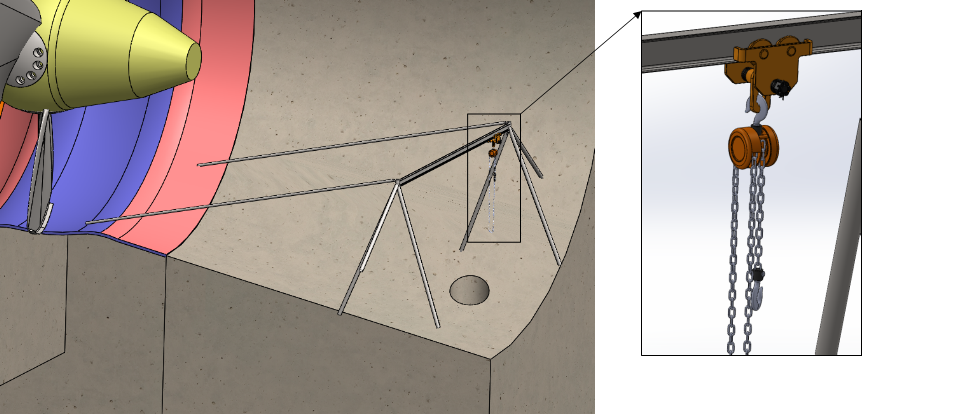
\includegraphics[width=0.8\columnwidth]{figs/bases/talha}
   \caption{Lifting structure}
   \label{fig::talha}
\end{figure}

\begin{figure}[h!]
   \centering
   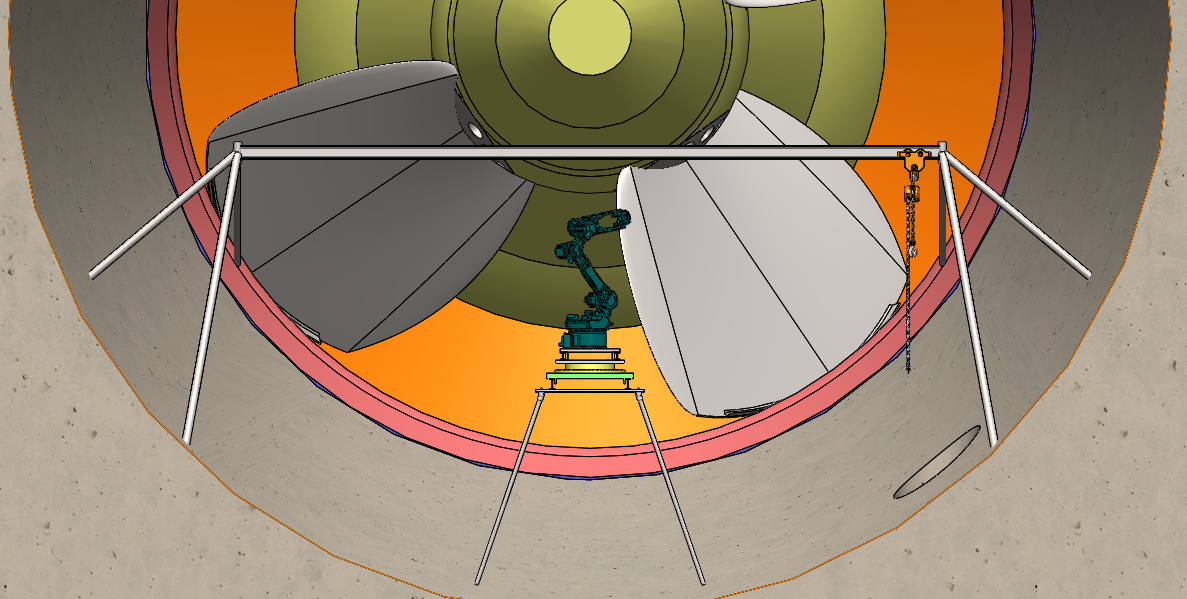
\includegraphics[width=0.8\columnwidth]{figs/bases/talha_trilho}
   \caption{Hoist and trolley - frontal point of view}
   \label{fig::talha_trilho}
\end{figure}

\subsection{Fixation}

Due to the dynamic forces of arm, the fixation of the structure on the
environment should be designed carefully. Because the water normally flow at
high pressures inside the draft tube and runner area, no permanent
infrastructure modifications are allowed. Thus any envisioned attachment method
should be removable without causing any damage to any surface.

In a technical visit carried out in October 2015 the
feasibility of magnetic attachment points for anchoring and fastening
were successfully tested.
The test aimed to verify the actual load limit on the magnet considering
the environment ( geometry ), materials and finishes on the actual surface.

Soldering is a fixation option for surfaces were the magnetic load limit is
not satisfatory, but it still a temporary solution and should be removed after
the hardcoating process.

% Devido aos esforços dinâmicos de operação do robô, a fixação da estrutura da
% base mecânica no ambiente deve ser dimensionada com cuidado. Por se
% tratar de um ambiente de escoamento de fluido sob pressão, não são admitidas
% modificações permanentes de infra-estrutura no interior da turbina, logo,
% qualquer método de fixação utlizado deve ser removível, sem causar nenhum dano
% à qualquer superfície. Em visita técnica realizada em Outrubro de 2015 foi
% testada a viabilidade de utlização de bases magnéticas para o sistema de
% ancoragem e fixação. Este teste teve o objetivo de verificar a real carga limite de tração
% do imã, considerando o ambiente (geometria), materiais e acabamentos
% superficiais reais a que estará submetido na solução final. O resultado
% detalhado do teste encontra-se no Apêndice~\ref{ape::magnetic}.
% 
% Outra opção para fixação provisória seria a soldagem da estrutura na
% superfície do túnel. Esta opção segue como uma alternativa ainda para regiões
% de difícil fixação da base magnética.